\label{sec:2_related_work}
\section{Related Work} 

% Computer vision
% ------------------------------------------
\subsection{Computer Vision}
Computer Vision is the interdisciplinary task of making computers understand and act on visual input. This scientific discipline's main objective is to make computers extract high-dimensional data from the real world, using digital images and videos. The extraction of visual information that can be used by computers includes methods for collecting, processing, analyzing, and understanding the images, using statistics, geometry, physics, and learning theory. 

% Object detection
Object detection is an important part of computer vision that has made astonishing progress. It has been an important topic of research because it is one of the fundamental problems in computer vision. Detecting objects form the fundamental basis of other computer vision tasks, such as object tracking, segmentation, and image captioning. A lot of these sub-domains achievements have come from using \gls{cnn} architectures with more layers, trained on larger datasets, and more powerful computers. These main components have made the algorithms capable to learn a deeper understanding of the visual world and learning more fundamental components of materials, objects, and scenes.  

% Is this relevant?
Krizhevsky et al. introduced AlexNet\cite{krizhevskyImageNetClassificationDeep2017}, as a variant of the \gls{cnn} proposed by LeCun et al.\cite{lecunHandwrittenDigitRecognition1989, lecunGradientbasedLearningApplied1998} seen in Figure \ref{fig:lenet}, both utilizing the backpropagation algorithm \cite{rumelhartLearningRepresentationsBackpropagating1986}
in training. The main difference is that AlexNet uses three more layers, ReLu \cite{fukushimaCognitronSelforganizingMultilayered1975}
, and is running on \glspl{gpu} instead of \glspl{cpu}, which in practice means more efficient use of computing power.
AlexNet achieved impressive results in the ImageNet \cite{dengImageNetLargeScaleHierarchical2009} 2012 Challenge and is often considered the most influential paper published in computer vision. 
Following this paper, there has been an increasing amount of work done and papers published in the domain of deep learning and images during the last decade.

\begin{figure}[htb]
    \centering
    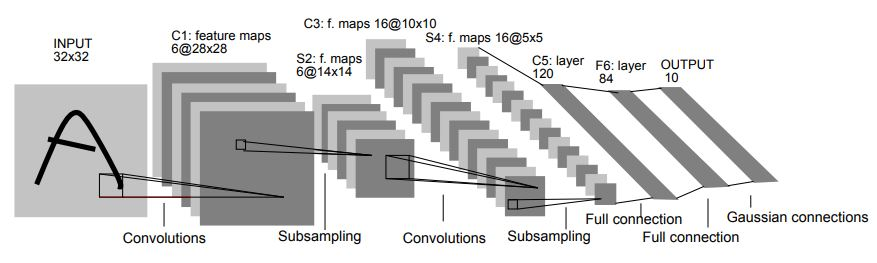
\includegraphics[width=12cm]{images/LeNet.jpg}
    \caption{\gls{cnn} architecture of LeNet-5 proposed by LeCun et al. \cite{lecunGradientbasedLearningApplied1998}.}
    \label{fig:lenet}
\end{figure} 

% XAI
% ------------------------------------------
\subsection{Explainable AI (XAI)}


% LIME
In the pursuit of a method that helps the explaining model to be locally faithful to the underlying model, Ribeiro et al. \cite{ribeiroWhyShouldTrust2016} proposed \gls{lime}. This method is model-agnostic and explains any method by learning an interpretable, less complex model locally around a specific prediction. This approach assures that the explanation is locally accurate and represents the actual inner workings of the model. 
In the same paper, they also introduce a method for explaining the global attributes of the model, by framing the task as a submodular optimization problem. The method is called SP-LIME (Submodular Pick LIME) and with this approach, they can achieve global explanations that are locally accurate and faithful to the underlying model in a non-redundant way.

% SHAP
Making non-redundant explanation features in a faithful and efficient way is not easy. Lundberg et al. \cite{lundbergUnifiedApproachInterpreting2017} proposed a unified framework for interpreting predictions made by the underlying method. This framework is called \gls{shap} and it assigns each feature a value of importance for a specific prediction. The framework utilizes the class of additive feature attribution methods and estimates the Shapley % cite
values from cooperative game theory, for that prediction. With this approach, they achieve explanations that are more effective to compute and/or have better consistency with human intuition than previously proposed methods.  


% Grad-CAM
Visually explaining features that contributed to an image prediction can be an important factor in gaining trust in a model. Selvaraju et al. \cite{selvarajuGradCAMVisualExplanations2020} proposed a technique for making \glspl{cnn} more explainable and transparent by producing visual explanations for the underlying model. The technique is called \gls{gradcam}, which is a generalization of CAM proposed by Zhou et al. \cite{zhouLearningDeepFeatures2016}, and uses the gradients in a single backtrack of any target concept. Therefore it does not need any architectural changes or retraining of the underlying prediction model to produce a localization map highlighting the important regions in the image for predicting the given concept, which is often called a saliency map in computer vision.

% DenseCap


% FLEX
While visual-only explanations can give the user insight into which areas of the image were important in making the decision, they tell little to nothing about why those regions were important. Linguistic descriptions on the other hand provide the user with an essential understanding of what the model evaluated when predicting. 
Wickramanayake et al. \cite{wickramanayakeFLEXFaithfulLinguistic2019} propose \gls{flex} to merge saliency maps with linguistic descriptions that are locally accurate. In this approach, they look at the gradients through layers and identify the activations that were most important in the single decision. The advantage of looking at different layers is that alongside getting an explanation that is faithful to the underlying model, they also extract features the \gls{cnn} identifies at each layer. A \gls{cnn} may represent high-level concepts, like a "car", at the last layer, while identifying features such as texture and color at earlier layers. In using the activations at all important layers, \gls{lime} achieves an image caption that explains all the important parts of the prediction using sentences. \gls{flex} maps words to neurons in the \gls{cnn} by looking at high activations of that neuron combined with a word from the caption during the training. For this, they are using a \gls{cnn} and two stacked \gls{lstm} \cite{hochreiterLongShorttermMemory1997} cells. % cite

% VQA dataset
To make the linguistic abilities of computers more robust, Agrawal et al. \cite{agrawalVQAVisualQuestion2016} proposed a new dataset called \gls{vqa}. This provides a large dataset with free-form and open-ended questions and answers coupled with images. These questions and answers target different areas of the images, including underlying context and background details. The goal of this dataset is to make models that can learn multi-modal knowledge of the visual and linguistic domain to get a more general and complete understanding of the world. Models that have done well in this dataset are often \glspl{cnn}, to get visual understanding, combined with an \gls{rnn} % cite
for linguistic knowledge.

